\section{Proces návrhu a výroby desky plošných spojů}
\subsection{Návrh DPS}
\todo[inline]{proces navrhu PCB (DRC hodnoty)}
\todo[inline]{proces vyroby PCB (CNC)}


\subsection{Výroba DPS}
Pro výrobu prototypů desek plošných spojů lze využít metodu vytváření
izolačních mezer v měděné vrstvičce pomocí CNC frézy. Jde o poměrně rychlou
metodu s minimem manuální práce. Stroj navíc provádí i navrtání děr, jejichž
počet i na poměrně jednoduchých DPS využívajících v maximální možné míře
součástek pro povrchovou montáž dosahuje několika stovek. Celý proces se obejde
bez nutnosti pracovat s korozivními chemikáliemi. Frézování oboustranných DPS
je možné, v takovém případě se ale zvyšuje náročnost postupu. Je totiž nutné
zachovat pozici referenčního bodu při otáčení desky.

\subsubsection{CNC fréza}
Levným CNC strojem splňujícím požadavky na přesnost, rozměry pracovního
prostoru a podporované funkce vhodným pro amatérské účely je stavebnice
prodávaná prodejci na platformě Aliexpress pod označením CNC~1610. Je tvořena
konstrukcí z hliníkových profilů a několika 3D tištěných částí. Po sestavení
získává uživatel stroj s pracovním prostorem \SI{160 x 100 x 40}{\milli\meter}
řízený svobodným firmware Grbl\footnote{\url{https://github.com/gnea/grbl}}.

\begin{figure}[htbp]
    \centering
    \missingfigure{CNC 1610}
    \caption{CNC fréza CNC~1610 s drobnými úpravami}
    \label{fig:CNC freza}
\end{figure}


\paragraph{Modifikace}
Po zakoupení stroje byly provedeny některé modifikace, které nadále
zjednodušují proces výroby DPS. Jednou z nich je přidání koncových spínačů.
Jejich funkce je dvojí. Zvyšují bezpečnost, protože zabraňují nárazu
pohyblivých částí stroje do jeho rámu (v případě využití
\foreignlanguage{english}{homing cycle} dokonce nemusí nutně dojít ani
k sepnutí tohoto spínače, pohyb mimo pracovní prostor je detekován výpočetně).
Umožňují také provést po spuštění stroje kalibraci
(\foreignlanguage{english}{homing cycle}), po které odpovídají souřadnice
stroje (v Grbl zvané \foreignlanguage{english}{machine coordinates})
konkrétním bodům v jeho pracovním prostoru. Díky tomu je možné beze ztráty
přesnosti obnovit práci například po výpadku napájení.

Druhá modifikace je pro výrobu DPS ještě důležitější. Jde o přidání kabelů
s krokosvorkami na vstup pro sondu (\foreignlanguage{english}{probe}). Jedna ze
svorek je spojena s měděnou vrstvou obráběné DPS, druhá je připojena na
frézovací nástroj upnutý v zastaveném vřetenu. Stroj díku tomu může přesně
změřit výšku desky v různých bodech a kompenzovat tak její průhyby. Vlastní
frézování je totiž velmi mělké, méně než \SI{200}{\micro\meter}.

\begin{figure}[htbp]
    \centering
    \missingfigure{CNC woodpecker board}
    \caption{%
        Řídicí elektronika CNC frézy s připojenými koncovými spínači a~sondou
    }
    \label{fig:CNC rizeni}
\end{figure}

Po provedení modifikací je nutné správně změnit nastavení Grbl, zejména
\verb|$5|, \verb|$6|, \verb|$20|, \verb|$21| a \verb|$22| až \verb|$27|.
Je také nutné správně nastavit rozměry pracovního prostoru (\verb|$130| až
\verb|$132|), protože výrobce toto nastavení ignoruje a ponechává jej na
výchozí hodnotě. Úplná konfigurace Grbl včetně vysvětlení jednotlivých
nastavení je otištěna v příloze~\vref{app:grbl config}.

Aby bylo možné využívat novější verzi řídicího software (spouštěného na
počítači), je nutné aktualizovat firmware stroje z verze Grbl~0.9j na
Grbl~1.1h. Aktualizace se provádí dle instrukcí na domovské stránce projektu
Grbl pomocí Arduino IDE. Přečtením obsahu paměti FLASH s původním firmware bylo
zjištěno, že použitý bootloader odpovídá desce \uv{Arduino nano (old
bootloader)}. Před aktualizací je vhodné vytvořit zálohu původního obsahu
paměti. To lze na počítači s operačním systémem GNU/Linux s nainstalovaným
Arduino IDE provést následujícím příkazem:
\begin{lstlisting}[style=terminal]
$ $HOME/.arduino15/packages/arduino/tools/avrdude/6.3.0-arduino17/bin/avrdude \
    -C$HOME/.arduino15/packages/arduino/tools/avrdude/6.3.0-arduino17/etc/avrdude.conf \
    -v -patmega328p -carduino -P/dev/ttyUSB0 -b5 7600 -D \
    -Uflash:r:$HOME/Desktop/CNC/GRBL-old-read.bin:r
\end{lstlisting}
Dále je nutné zazálohovat nastavení Grbl, která jsou uložená v paměti EEPROM.
To se provádí připojením terminálu na sériový port stroje a spuštěním příkazu
\verb|$$|.
Po aktualizaci firmware je potřeba nová nastavení stroje porovnat s touto
zálohou a příslušně je upravit.

\paragraph{Nástroje}
Pro frézování obrazce DPS jsou vhodné nástroje ve tvaru V. Průměr nástroje
v místě upnutí je \SI{3,175}{\milli\meter}, to je standardní rozměr používaný
na malých CNC frézách. Nástroj se poté zužuje s úhlem
\SI{30}{\degree}\todo{nebo 15?} až k velmi tenkému hrotu.

Pro vrtání děr využíváme tvrzené vrtáky o průměru \SI{0,8}{\milli\meter}
a \SI{1}{\milli\meter}. Tyto dva rozměry postačí pro naprostou většinu běžných
DPS.
\todo{dopsat nastroje}


\paragraph{Řídicí software}
Řízení vlastního stroje (krokových motorů a vřetena) je řešeno mikrokontrolérem
na jeho desce s řídicí elektronikou. Jeho firmware Grbl implementuje jazyk
G-kód, příkazy jsou přijímány na sériovém portu. Tyto příkazy by bylo možné
zasílat z běžného terminálu, pro zvýšení pohodlí při obsluze stroje je ale
vhodné využít specializovaný software. Jedním z takových programů je
Candle\footnote{\url{https://github.com/Denvi/Candle}}. Jde o svobodný software
distribuovaný pod licencí GNU GPL v3.0. Kromě GNU/Linux je podporován
i operační systém Microsoft Windows. Uživatelské rozhraní tohoto programu (viz
obrázek~\vref{fig:CNC Candle} velmi dobře funguje s dotykovým monitorem.
Jednoduché operace je možné provádět přímo dedikovanými tlačítky či klávesovými
zkratkami, složitější příkazy je možné vypisovat přímo do okna \uv{Console}.

% Stabilní verze z větve \gitbranch{master} je již poměrně stará, proto je
% využívána vývojová verze z větve \gitbranch{Experimental}.
% https://github.com/Denvi/Candle/issues/488#issuecomment-858985048

\begin{figure}[htbp]
    \centering
    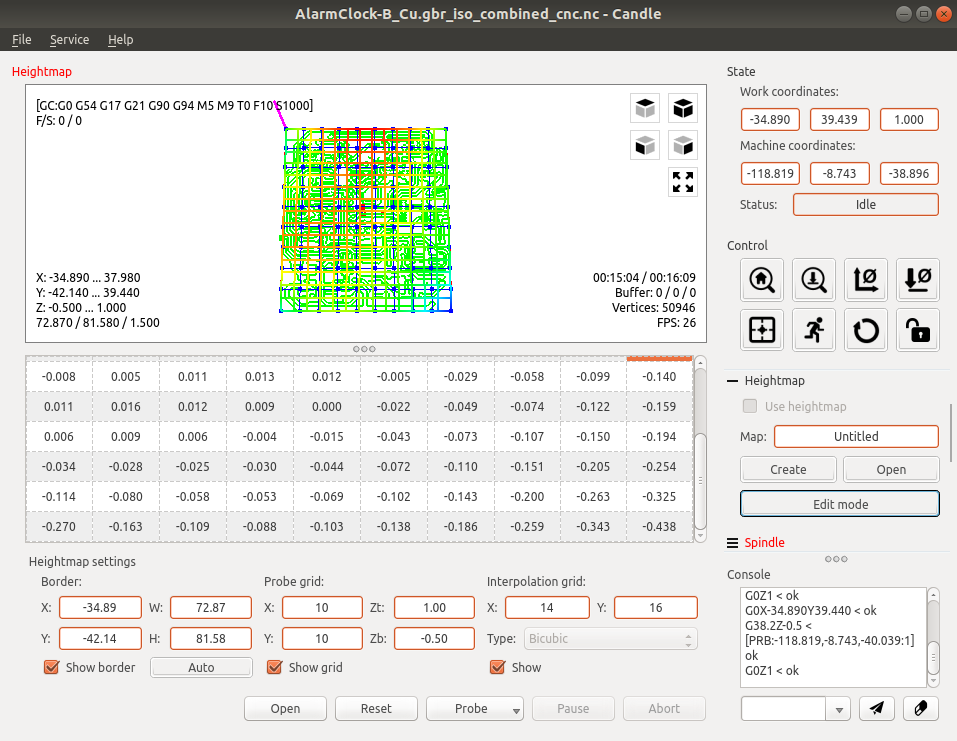
\includegraphics[width=\textwidth]{Candle-UI}
    \caption{Uživatelské rozhraní programu Candle}
    \label{fig:CNC Candle}
\end{figure}


\subsubsection{Generování G-kódu}
G-kód lze psát ručně pomocí běžného textového editoru. Mnohdy je to dokonce
nejrychlejší metoda. Jednoduché operace, jako například vyříznutí hotové DPS
z větší cuprextitové destičky, obvykle sestávají z méně než 15 příkazů
a operátor se základní znalostí G-kódu je zvládne vytvořit velmi rychle.
Složitější operace, jako například frézování vlastního obrazce DPS, ale
vyžadují desítky tisíc příkazů a jejich ruční tvorba by byla prakticky nemožná.
Existuje ale svobodný software FlatCAM\footnote{\url{http://flatcam.org/}},
který slouží k automatickému generování G-kódu z podkladů ve formátu Gerber.
\todo{FlatCAM}
